% Almansur_Crosswind_Project.tex
% Every number in this report is produced by src/viz/report_experiment.py and
% src/viz/report_figures.py (data in report/data, figures in report/figures).
% Compile with pdfLaTeX, twice, from the project root (or on Overleaf with the
% report/figures folder uploaded alongside this file).
\documentclass[10pt,a4paper]{article}

\usepackage[T2A,T1]{fontenc}
\usepackage[utf8]{inputenc}
\usepackage{lmodern}
\usepackage[margin=2.5cm]{geometry}
\usepackage{amsmath,amssymb}
\usepackage{graphicx}
\usepackage{booktabs}
\usepackage{caption}
\usepackage{subcaption}
\usepackage{float}
\usepackage{xcolor}
\usepackage{fancyhdr}
\usepackage[hidelinks]{hyperref}

\graphicspath{{report/figures/}}
\captionsetup{font=small,labelfont=bf}
\setlength{\parskip}{0.35em}
\setlength{\parindent}{1.2em}

\newcommand{\shorttitle}{Autonomous Crosswind Landing \& Flight Control}
\pagestyle{fancy}
\fancyhf{}
\fancyhead[L]{\small\shorttitle}
\fancyhead[R]{\small A.\ Jumabay}
\fancyfoot[C]{\small\thepage}
\renewcommand{\headrulewidth}{0.4pt}
\setlength{\headheight}{14pt}

\hypersetup{
  pdftitle={Autonomous Crosswind Landing and Flight Control System},
  pdfauthor={Almansur Jumabay}
}

\title{\vspace{-1.5em}\textbf{Autonomous Crosswind Landing \& Flight Control System:\\
Predictive Aerodynamic Disturbance Compensation in a 6-DoF Simulation Framework,
with a Proposed Hardware-in-the-Loop Extension}}
\author{Almansur Jumabay ({\fontencoding{T2A}\fontfamily{cmr}\selectfont Альмансур Джумабай})\\
\small 11th Grade Student, Dostyq School, Astana, Kazakhstan}
\date{30 October 2026}

\begin{document}
\maketitle
\thispagestyle{fancy}

\begin{abstract}
\noindent
Crosswind landing is demanding because the aircraft must fly a crabbed approach,
then remove the crab within seconds of touchdown while wind shear and gusts
disturb it. This report presents a simulation study of autonomous crosswind
landing using a nonlinear six-degree-of-freedom model of a Cessna-172-class
aircraft with a Dryden turbulence model, discrete gusts, wind shear and landing
gear contact. Three controllers are compared: a classical cascaded autoland, a
residual proximal policy optimisation (PPO) policy that corrects that autoland,
and the same policy under a Simplex runtime-assurance monitor with a one-second
look-ahead. Across 300 Monte-Carlo landings for the classical and supervised
controllers, the analytic crab angle agrees with simulation within
\(1.4^\circ\), and mean touchdown centreline error stays below \(3\)\,m even at a
\(20\)\,m/s crosswind. However, the interim policy, frozen at 800\,000 steps of a
planned 5\,000\,000, does not yet outperform the baseline: at \(10\)\,m/s both land
successfully in 19 of 30 trials, with hard landings the dominant failure. Under a
scripted \(20\)\,m/s lateral gust, 19 of 20 trials land with either controller.
A control decision costs under \(1\)\,ms on a desktop CPU, far below the \(50\)\,ms
control period. A browser-based WebGL console replays the recorded telemetry.
Hardware-in-the-loop integration is presented as a proposed design only; it has
not been built or tested, and no result here comes from physical hardware.
\end{abstract}

\section{Introduction and Aerodynamic Problem Statement}

On final approach a crosswind forces a pilot or autopilot to choose between two
incompatible goals. Tracking the centreline requires the nose to point into the
wind, whereas the landing gear requires the fuselage to align with the runway at
contact. The conventional solution is to fly a crabbed approach and remove the
crab in the flare, using rudder for alignment and a wing-low bank to hold the
centreline~\cite{stevens2015}. The manoeuvre takes place within a few metres of
the ground, where the bank margin before a wingtip strike is smallest.

Low-altitude wind makes this harder in two ways. First, the mean wind grows with
height and its direction veers, so the required crab changes during the descent.
Second, turbulence and discrete gusts perturb airspeed, sideslip and angle of
attack at frequencies close to those of the closed-loop modes~\cite{milf8785c}.
Fixed-gain PID loops respond to the error after it has developed. They are
straightforward to tune around a trim point, but their gains do not adapt to the
current gust environment. Section~\ref{sec:results} shows how this appears here:
the classical autoland holds the centreline well, yet its touchdown sink rate
degrades quickly as the wind grows.

This motivates two questions: can a learned policy reduce these failures by
correcting a competent classical controller, and can it be used without
surrendering safety? The project combines residual reinforcement
learning~\cite{silver2018residual,johannink2019residual} with a Simplex
runtime-assurance architecture~\cite{sha2001simplex}. ``Predictive'' has a precise
and limited meaning in this report: the monitor extrapolates the state one second
ahead and the autoland estimates the wind continuously from air data. This is not
model predictive control and no gust is forecast before it arrives.

\section{Mathematical Kinematics and Aerodynamic Modelling}

The integrated state is
\(\mathbf{x}=[\mathbf{p}^n,\mathbf{v}^b,\mathbf{q},\boldsymbol{\omega}^b]^\top\in\mathbb{R}^{13}\),
with position in a runway-fixed North-East-Down frame, velocity and rates in body
axes, and a unit attitude quaternion. Translational and rotational dynamics are
\begin{align}
\dot{\mathbf{v}}^b &= \frac{1}{m}\left(\mathbf{F}_A+\mathbf{F}_T+\mathbf{F}_G
 + R_{nb}^\top[0,\,0,\,mg]^\top\right)-\boldsymbol{\omega}^b\times\mathbf{v}^b, \label{eq:trans}\\
\dot{\boldsymbol{\omega}}^b &= I^{-1}\left(\mathbf{M}_A+\mathbf{M}_G-\boldsymbol{\omega}^b\times I\boldsymbol{\omega}^b\right), \label{eq:rot}
\end{align}
integrated by fourth-order Runge--Kutta at \(\Delta t=0.01\)\,s, with the controller
acting at 20\,Hz. Aerodynamic coefficients, a smooth stall blend~\cite{beard2012}
and McCormick ground effect~\cite{mccormick1995} depend on the wind through the
air-relative velocity \(\mathbf{v}_r=\mathbf{v}^b-R_{nb}^\top\mathbf{w}^n\). The
mean wind follows a shear and veer profile referenced to 20\,ft,
\begin{equation}
W(h)=W_{20}\left(\frac{h}{6.096}\right)^{1/7},\qquad
\chi(h)=\chi_{20}+k_{\mathrm{veer}}\frac{h-6.096}{100},
\label{eq:shear}
\end{equation}
to which Dryden turbulence~\cite{milf8785c} and Poisson-triggered 1-cosine gusts,
\(\mathbf{w}_g(t)=\tfrac{1}{2}\mathbf{A}\bigl(1-\cos(2\pi(t-t_0)/T)\bigr)\), are
added. Table~\ref{tab:params} lists the parameters taken from
\texttt{AircraftParameters} and \texttt{EnvConfig}. The automated test suite, which
currently passes all 40 tests, checks integrator convergence order, conservation of
angular momentum and energy, and turbulence statistics.

\begin{table}[H]
\centering
\caption{Simulation parameters extracted from \texttt{src/env/aircraft\_env.py}.}
\label{tab:params}
\small
\begin{tabular}{@{}llll@{}}
\toprule
Parameter & Value & Parameter & Value\\
\midrule
Mass \(m\) & 1043 kg & Approach speed \(V_{\mathrm{ref}}\) & 33 m/s\\
Wing area \(S\) & 16.2 m\(^2\) & Glideslope & \(3^\circ\)\\
Span \(b\) / chord \(c\) & 10.92 / 1.49 m & Runway length / width & 1600 / 30 m\\
\(I_{xx},I_{yy},I_{zz}\) & 1285, 1825, 2667 kg\,m\(^2\) & Surface lag / rate limit & 0.06 s / \(80^\circ\)/s\\
\(C_{n_\beta},\,C_{n_{\delta_r}}\) & 0.065, \(-0.0657\) & Crash sink-rate limit & \(-1.5\) m/s\\
\(C_{l_\beta},\,C_{l_{\delta_a}}\) & \(-0.089\), 0.178 & Rudder / aileron limit & \(\pm25^\circ\) / \(\pm20^\circ\)\\
\bottomrule
\end{tabular}
\end{table}

\subsection{Crab Angle}

For a steady, wings-level approach with zero sideslip and a ground track on the
centreline, the lateral air velocity must cancel the crosswind, which gives the
heading correction
\begin{equation}
\beta_{c}=\arcsin\left(\frac{v_{\mathrm{cross}}}{v_{\mathrm{air}}}\right).
\label{eq:crab}
\end{equation}
The subscript distinguishes this crab angle from the aerodynamic sideslip
\(\beta=\arcsin(v_r/V_a)\) used in the code. Equation~\eqref{eq:crab} was verified
against the simulator in turbulence-free air by comparing it with the mean heading
error flown by the autoland between 30 and 50\,m. Table~\ref{tab:crab} shows
agreement within \(1.4^\circ\), with the gap growing with wind speed.

\begin{table}[H]
\centering
\caption{Analytic crab angle, Eq.~\eqref{eq:crab}, against the simulated value (no turbulence or gusts, \(h\in[30,50]\) m; \(v_{\mathrm{cross}}\) and \(v_{\mathrm{air}}\) evaluated locally).}
\label{tab:crab}
\small
\begin{tabular}{@{}lcccccc@{}}
\toprule
\(W_{20}\) [m/s] & 2.5 & 5.0 & 7.5 & 10.0 & 12.5 & 15.0\\
\midrule
Predicted \(\beta_c\) [deg] & 5.65 & 11.24 & 16.80 & 22.37 & 27.97 & 33.61\\
Simulated [deg] & 5.72 & 11.42 & 17.18 & 22.99 & 28.90 & 34.96\\
\bottomrule
\end{tabular}
\end{table}

\subsection{De-crab and Flare}

For analysis, the lateral-directional dynamics about the approach condition can be
written in the standard small-perturbation form with
\(\mathbf{x}_{\mathrm{lat}}=[\beta,\,p,\,r,\,\phi]^\top\) and
\(\mathbf{u}=[\delta_a,\,\delta_r]^\top\):
\begin{equation}
\dot{\mathbf{x}}_{\mathrm{lat}}=
\begin{bmatrix}
Y_\beta/V & 0 & -1 & g/V\\
L_\beta & L_p & L_r & 0\\
N_\beta & N_p & N_r & 0\\
0 & 1 & 0 & 0
\end{bmatrix}\mathbf{x}_{\mathrm{lat}}+
\begin{bmatrix}
0 & Y_{\delta_r}/V\\
L_{\delta_a} & L_{\delta_r}\\
N_{\delta_a} & N_{\delta_r}\\
0 & 0
\end{bmatrix}\mathbf{u}.
\label{eq:ss}
\end{equation}
At \(V=33\)\,m/s and sea level, with \(\bar{q}Sb\approx1.18\times10^{5}\)\,N\,m and
neglecting products of inertia, the table values give
\(N_\beta\approx2.88\)\,s\(^{-2}\), \(N_{\delta_r}\approx-2.91\)\,s\(^{-2}\),
\(L_\beta\approx-8.17\)\,s\(^{-2}\) and \(L_{\delta_a}\approx16.3\)\,s\(^{-2}\).
Since \(|N_\beta|\approx|N_{\delta_r}|\), holding a sideslip \(\beta\) in steady
flight needs about the same rudder angle, so the 12-degree sideslip limit below sits
well inside the \(25^\circ\) rudder limit. Model~\eqref{eq:ss} is used for this
reasoning only; the simulator integrates the full nonlinear equations.

Below a wheel height of 4\,m the autoland commands alignment and a wing-low bank:
\begin{align}
\delta_r &= k_\psi(\psi_e-\psi_{\mathrm{res}})+k_r r, &
\psi_{\mathrm{res}} &= \operatorname{sgn}(\psi_e)\max\left(|\psi_e|-12^\circ,\,0\right),\label{eq:decrab}\\
\delta_a &= k_\phi(\phi_{\mathrm{cmd}}-\phi)-k_p p, &
\phi_{\mathrm{cmd}} &= \operatorname{sat}_{\pm8^\circ}\left(-0.54\,\dot{y}-0.01\,y\right),\label{eq:winglow}
\end{align}
with \(k_\psi=2.0\), \(k_r=0.4\), \(k_\phi=1.2\) and \(k_p=0.15\) (angles in radians,
\(\psi_e\) the heading error latched for \(\psi_{\mathrm{res}}\) at de-crab entry).
Limiting the commanded alignment leaves a small residual crab in strong wind rather
than demanding a sideslip that would lose lift. Below 10\,m an exponential flare
commands \(\dot{h}_{\mathrm{cmd}}=-h_w/2.8-0.25\)\,m/s, and an angle-of-attack
protection caps the pitch command to keep \(\alpha\) below \(12^\circ\).

\subsection{Multi-Objective Loss}

The policy is trained by maximising a reward rather than minimising an explicit loss.
Writing the dense part as \(L=-r\) and grouping its terms gives the requested form,
\begin{equation}
L_{\mathrm{total}}=w_1L_{\mathrm{glide}}+w_2L_{\mathrm{yaw}}+w_3L_{\mathrm{structural}},
\qquad w_1=2.0,\quad w_2=0.05,\quad w_3=0.4,
\label{eq:loss}
\end{equation}
where the weights are the leading coefficients in \texttt{RewardConfig}. This grouping
is a presentation of the implemented terms; the code has no single scalar triple. With
\(\rho(e)=\sqrt{1+e^2}-1\), \(\Lambda_H=(1-h/H)_+\) and tolerances that widen with
the distance \(d\) to the aim point,
\begin{align}
L_{\mathrm{glide}}&=\rho\left(\frac{e_{gs}}{4+0.03d}\right)+\rho\left(\frac{y}{6+0.02d}\right)+\frac{|d|}{2000},\label{eq:lglide}\\
L_{\mathrm{yaw}}&=\Lambda_{15}\left[\left(\frac{\psi_e}{5^\circ}\right)^2+\left(\frac{\dot{y}}{2}\right)^2\right],\label{eq:lyaw}\\
L_{\mathrm{structural}}&=\Lambda_{12}\left(-0.8-\dot{h}\right)_+^2+0.025\lVert\boldsymbol{\omega}\rVert^2+0.005\lVert\mathbf{a}\rVert^2+0.05\lVert\Delta\mathbf{a}\rVert^2.\label{eq:lstruct}
\end{align}
\(L_{\mathrm{glide}}\) enters as a potential-based shaping term, which preserves the
optimal policy~\cite{ng1999shaping}. A sparse touchdown reward and crash penalties
are added, and smaller attitude, airspeed and stall-protection penalties are omitted here for brevity. Lateral structural load is not penalised directly: crab, lateral speed and
sink rate act as surrogates, and the lateral load factor is measured afterwards
(Section~\ref{sec:results}).

\section{System Architecture and Technology Stack}

\paragraph{Software core.} The simulator is a Gymnasium environment in Python and
NumPy. Policies use PPO~\cite{schulman2017ppo} from Stable-Baselines3~\cite{raffin2021sb3}
on PyTorch, with separate \([256,256]\) tanh networks and a 23-dimensional observation
that contains air data but not the wind vector. In residual mode the applied action is
\(\mathbf{a}=\operatorname{clip}(\mathbf{a}_{\mathrm{autoland}}+0.3\,\mathbf{a}_{\mathrm{policy}})\).
The curriculum raises wind severity from 0.2 to 1.0 over 2\,000\,000 steps, while
evaluation uses full severity. The Simplex monitor checks bank, pitch, angle of attack,
airspeed, sink rate and path deviation against altitude-scheduled limits. On a predicted
violation, authority \(\lambda\) in \(\mathbf{a}=\lambda\mathbf{a}_{\mathrm{primary}}+(1-\lambda)\mathbf{a}_{\mathrm{fallback}}\)
blends to the fallback at 2.5\,s\(^{-1}\) and is latched for 3\,s; inside 15\,m it is
never handed back.

\paragraph{Frontend and 3D visualisation.} A React and Three.js console built with
WebGL replays recorded 20\,Hz rollouts with Catmull--Rom interpolation (Fig.~\ref{fig:console}).
It does not re-simulate in the browser. The rendered airliner is a procedural Blender
model with a fictional livery, whereas the flight data come from the Cessna-class
simulator, so the console is a visualisation and not evidence of airliner performance.

\begin{figure}[H]
\centering
\begin{subfigure}[t]{0.49\textwidth}
  \centering
  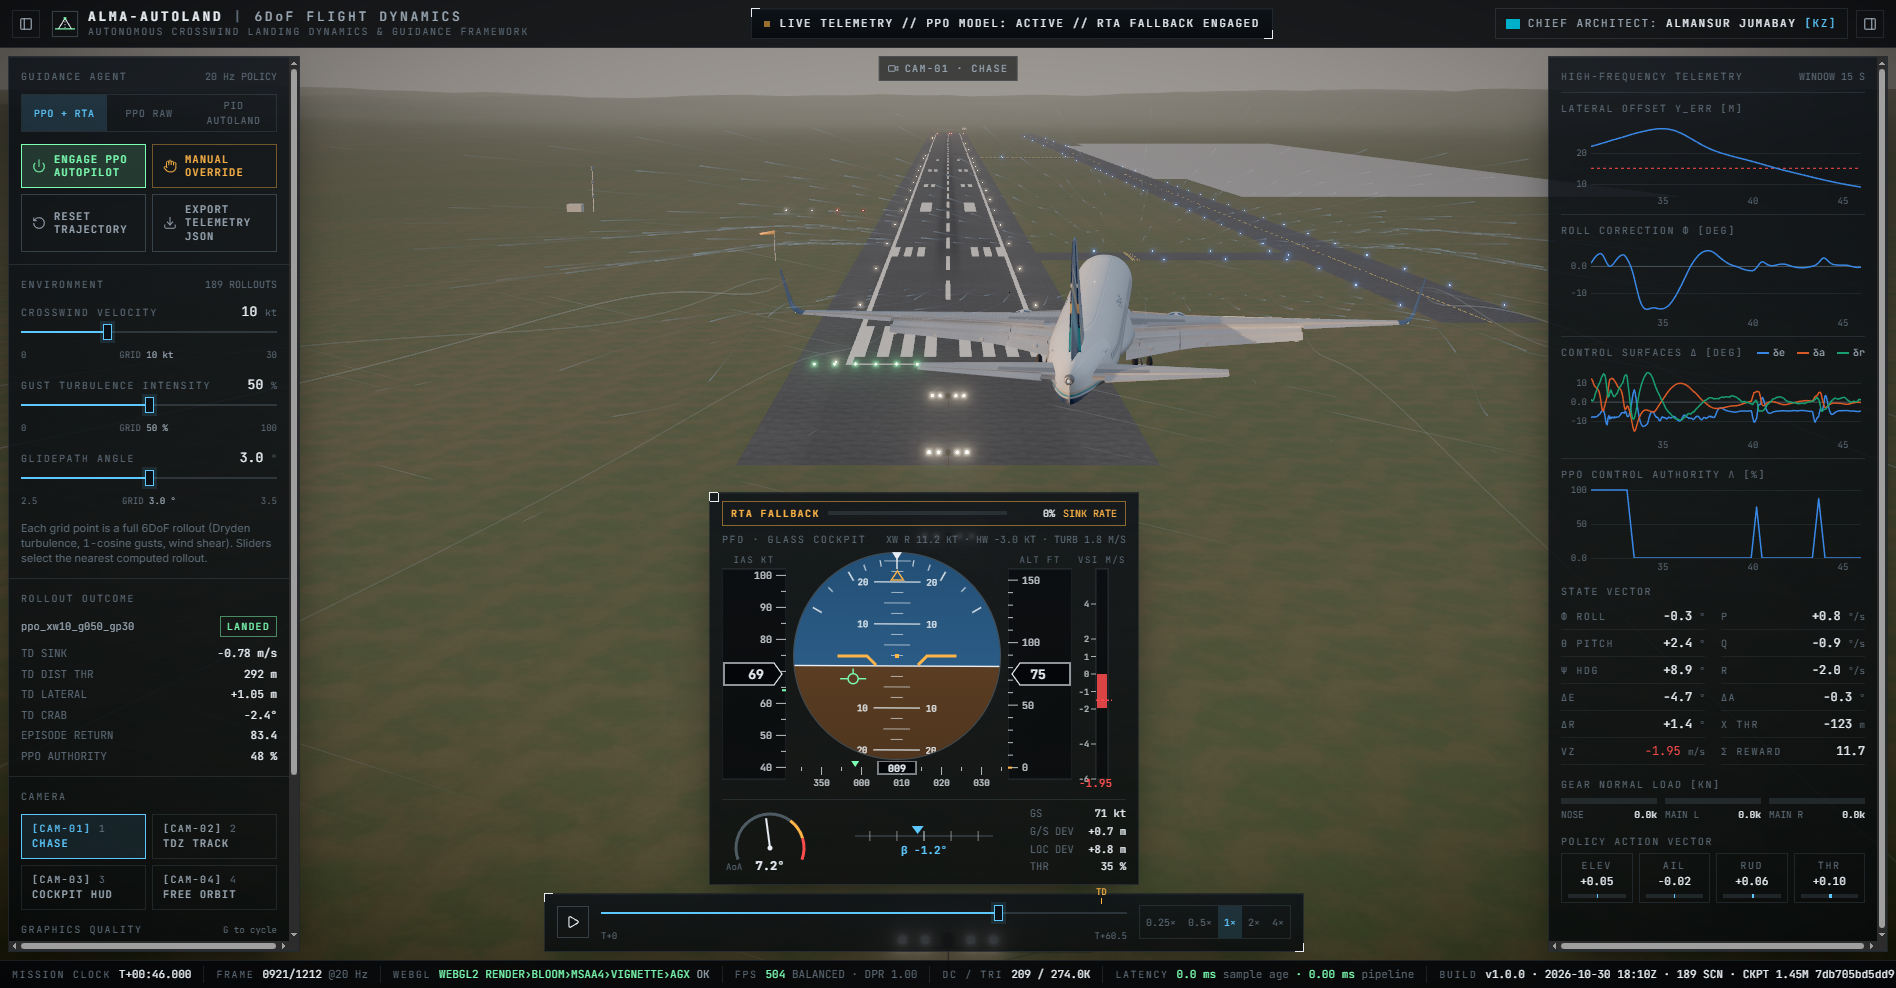
\includegraphics[width=\linewidth]{console_chase.png}
  \caption{Runway-referenced chase view, instruments and telemetry.}
\end{subfigure}\hfill
\begin{subfigure}[t]{0.49\textwidth}
  \centering
  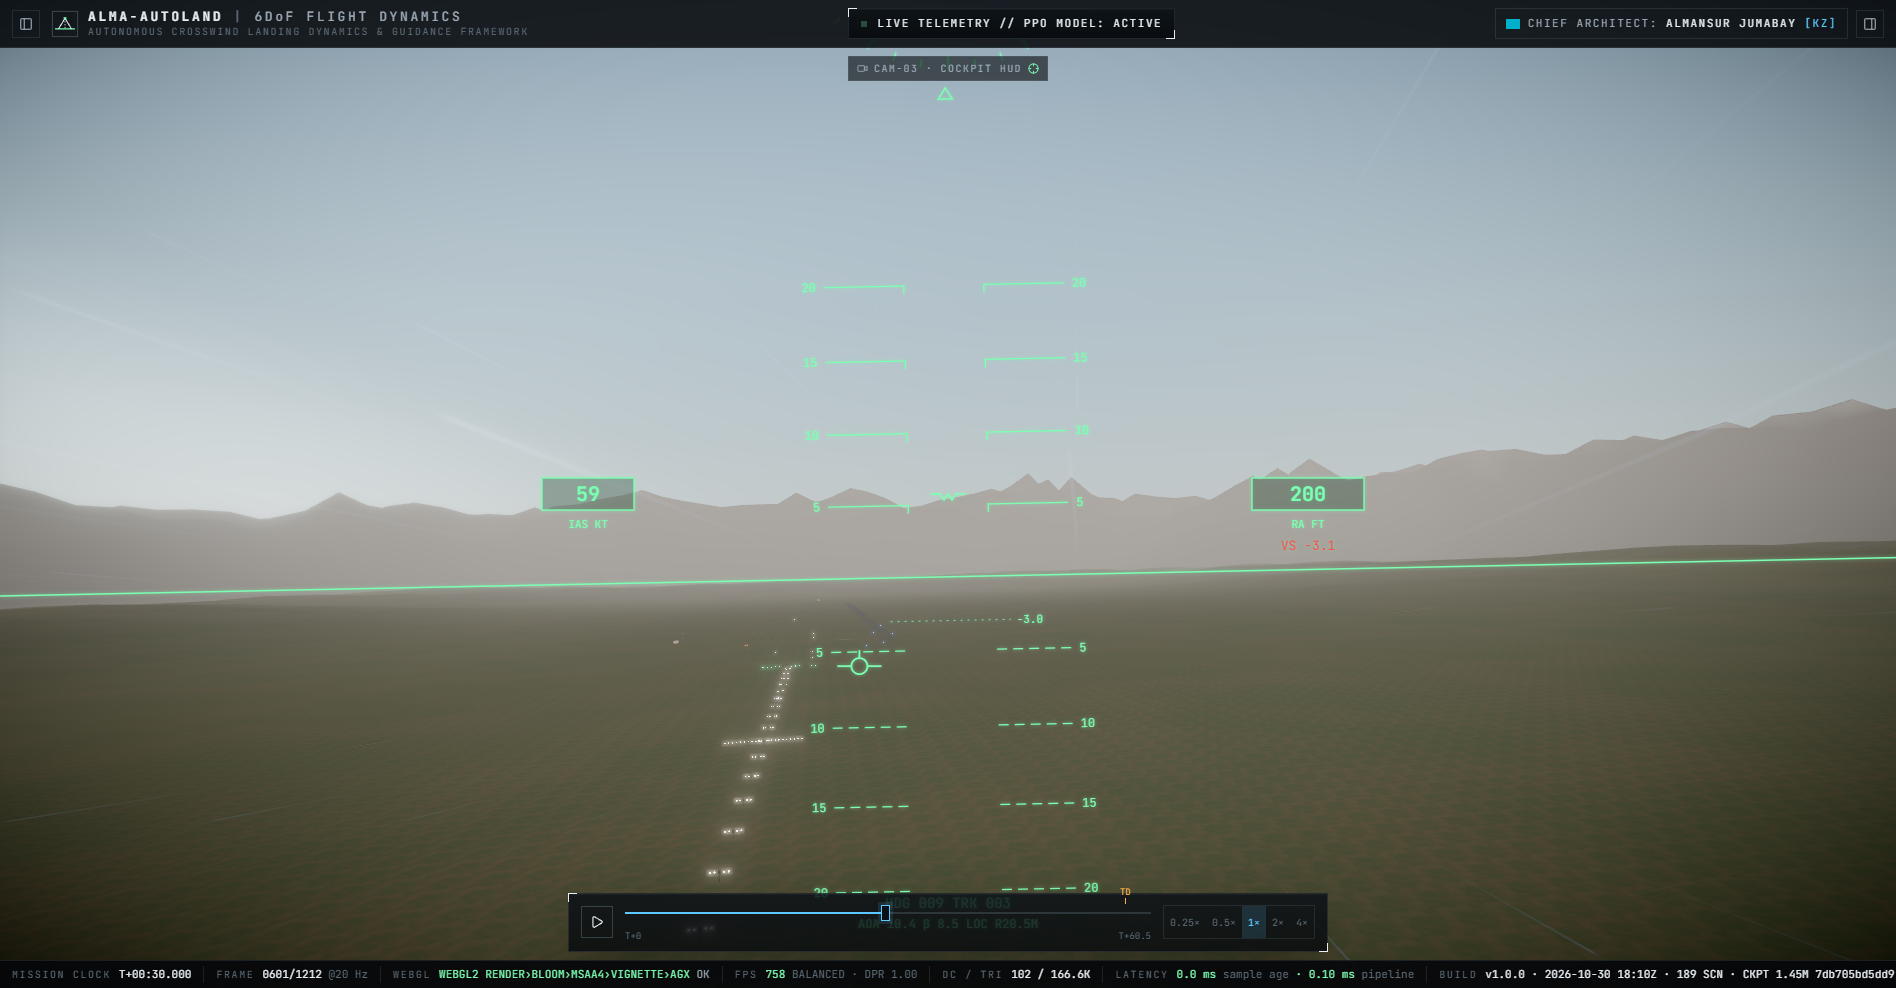
\includegraphics[width=\linewidth]{console_hud.png}
  \caption{Cockpit head-up display with flight-path vector.}
\end{subfigure}
\caption{WebGL mission console replaying simulator telemetry. The airframe is a visual model only; see the text.}
\label{fig:console}
\end{figure}

\paragraph{Hardware-in-the-loop integration (proposed, not implemented).} The repository
contains no firmware, serial code or sensor data, so this subsection is a design
proposal. HIL testing places real components in a simulated loop to expose timing and
sensor effects before flight~\cite{isermann1999hil}. The proposed bench would mount an
MPU-6050 six-axis IMU on an ESP32 or Arduino board, streaming attitude rates to the
browser through the Web Serial API. A first experiment would compare measured IMU rates
with commanded simulator motion on a manually driven gimbal; closing the loop with
servo-driven surfaces would follow. Expected risks include MEMS gyroscope drift,
vibration noise, and serial jitter against the 50\,ms control period. None of these
effects has yet been measured.

\section{Experimental Telemetry, Measurements and Data Visualisation}
\label{sec:results}

All results are from simulation. The tested policy is a snapshot of the residual run,
selected as the best evaluation at step 800\,000 (return \(101.1\pm18.5\) over 20
episodes, file hash \texttt{956d354f3845}). Training continues towards 5\,000\,000 steps,
so these are interim results. Controllers share the same random seeds in every test.
Figure~\ref{fig:training} shows evaluation returns. The absolute policy, which commands
the surfaces directly, remains erratic, supporting the move to a residual formulation.
The two returns are not strictly comparable, since the reward changed between the runs.

\begin{figure}[H]
\centering
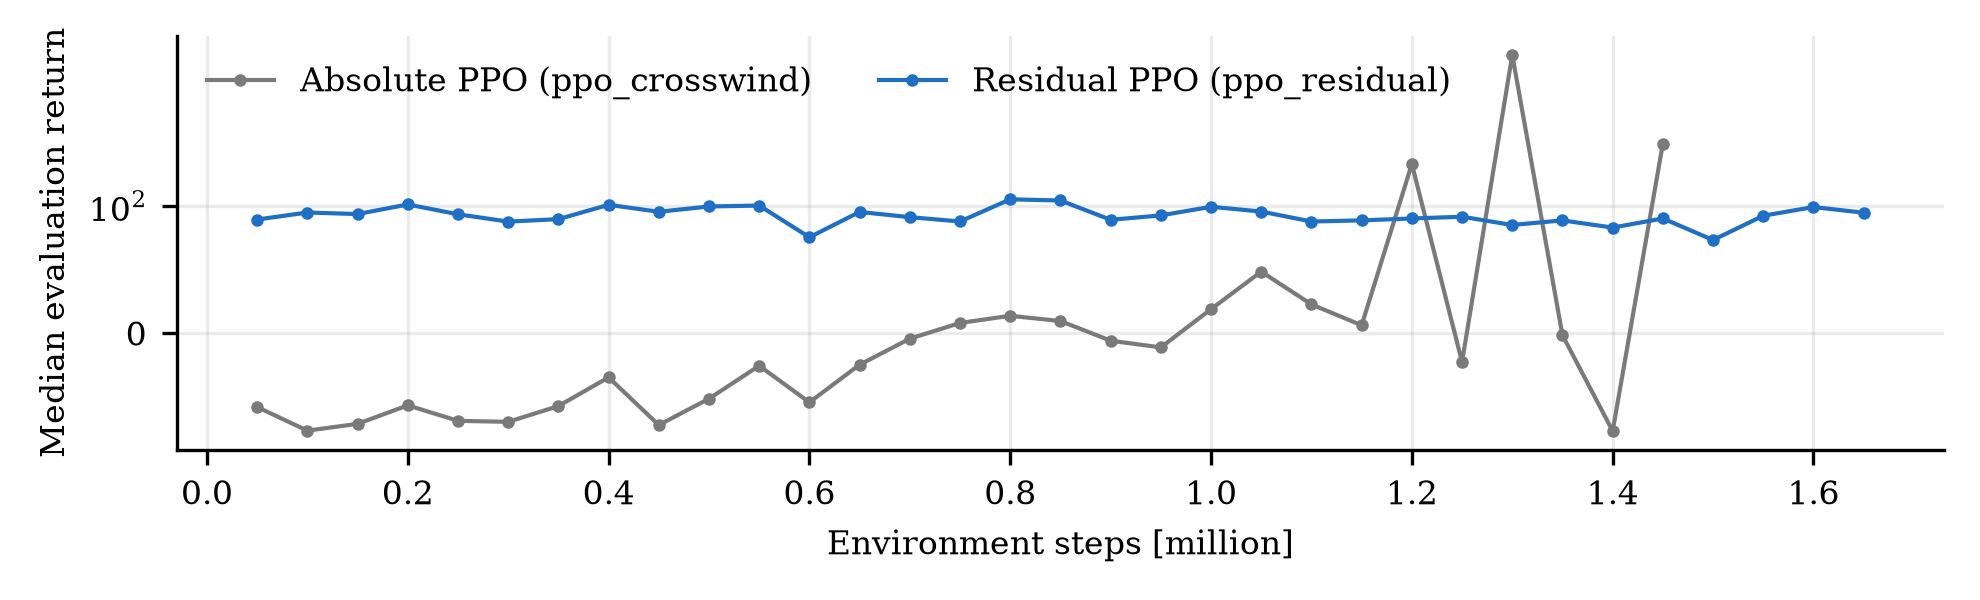
\includegraphics[width=0.92\textwidth]{training.png}
\caption{Median evaluation return against training steps at full wind severity (symmetric-log axis). Residual steps beyond 250\,000 come from the resumed run.}
\label{fig:training}
\end{figure}

\paragraph{Gust response.} A scripted lateral 1-cosine gust with a \(20\)\,m/s peak and
a 120\,m wavelength (about 3.5\,s) was applied at \(x=-800\)\,m, roughly 58\,m above
ground, on top of a \(5\)\,m/s mean crosswind and Dryden turbulence, for 20 seeds per
controller. Figure~\ref{fig:gust} shows the pitch, roll and heading response. The median
peak lateral deviation was 2.8\,m for the classical autoland and 3.0\,m with the policy
and monitor, and bank first moved by \(2^\circ\) about 1.4\,s after gust onset in each
case. This is a transient at a safe height, so it does not test a gust in the flare.

\begin{figure}[H]
\centering
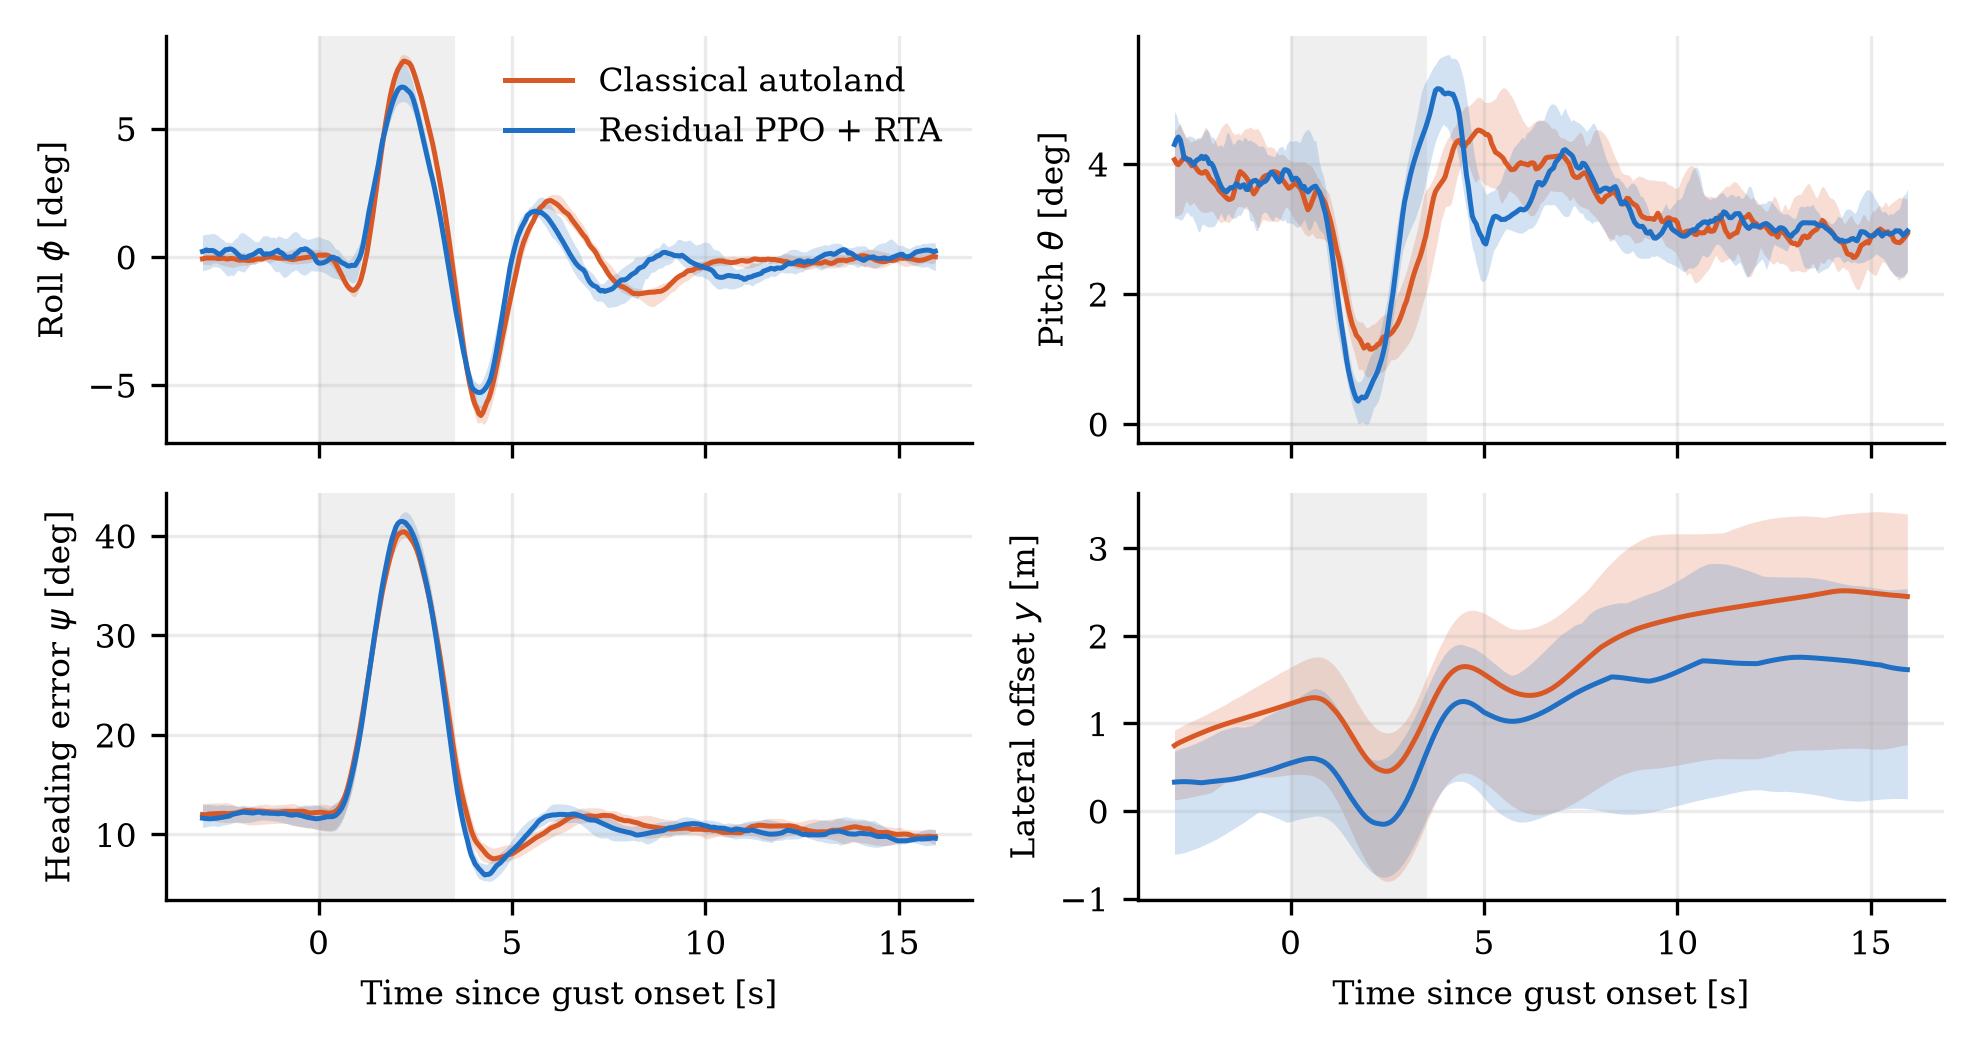
\includegraphics[width=0.92\textwidth]{gust_response.png}
\caption{Response to a 20\,m/s peak lateral gust (grey band). Lines are medians over 20 seeds and shaded regions the interquartile range.}
\label{fig:gust}
\end{figure}

\paragraph{Monte-Carlo sweep.} Each controller flew 30 landings per mean crosswind with
randomised initial offsets, turbulence and random gusts (Fig.~\ref{fig:mc}, Table~\ref{tab:compare}).
The lateral load factor \(n_y\) is the peak body-axis lateral specific force within 1\,s
of touchdown, sampled at 20\,Hz, so short gear transients may be under-reported. The
requested comparison ``without'' the system uses the classical autoland as the baseline,
which is itself autonomous; no human-pilot or uncontrolled baseline was measured.

\begin{figure}[H]
\centering
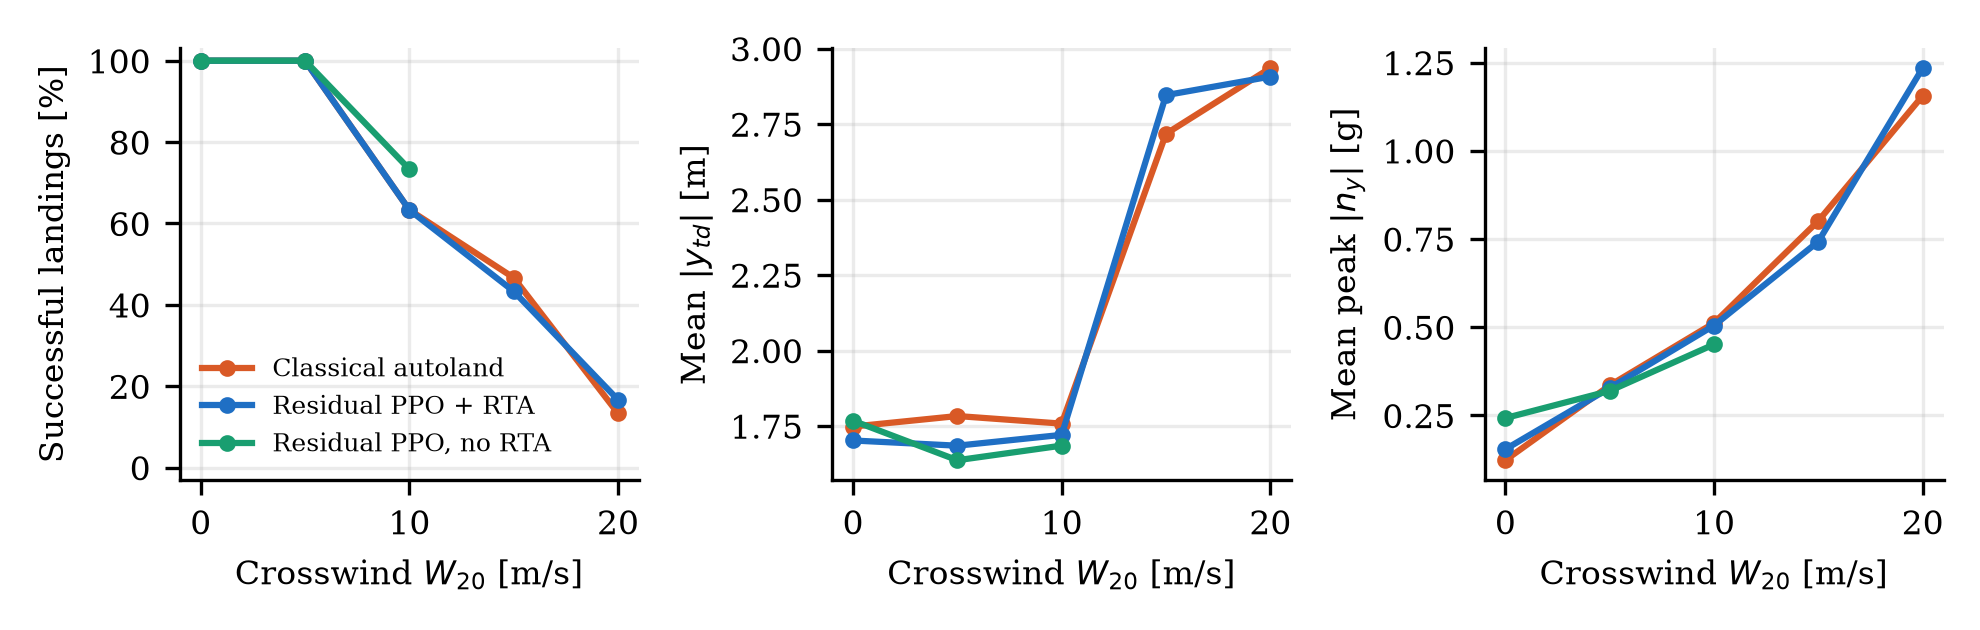
\includegraphics[width=0.98\textwidth]{monte_carlo.png}
\caption{Monte-Carlo results per crosswind. The unprotected policy has data only up to 10\,m/s because the run was stopped early.}
\label{fig:mc}
\end{figure}

\begin{table}[H]
\centering
\caption{Performance comparison (30 landings per entry unless stated). \(|y_{td}|\) and \(n_y\) average the trials that reached the ground. ``--'' means not measured.}
\label{tab:compare}
\small
\begin{tabular}{@{}llcccc@{}}
\toprule
Condition & Controller & Landed & Mean \(|y_{td}|\) [m] & Mean \(n_y\) [g] & Mean \(\dot{h}_{td}\) [m/s]\\
\midrule
\(W_{20}=5\) m/s & Classical autoland & 30/30 & 1.78 & 0.34 & \(-0.65\)\\
 & Residual PPO + RTA & 30/30 & 1.69 & 0.33 & \(-0.62\)\\
 & Residual PPO, no RTA & 30/30 & 1.64 & 0.32 & \(-0.68\)\\
\midrule
\(W_{20}=10\) m/s & Classical autoland & 19/30 & 1.76 & 0.51 & \(-1.40\)\\
 & Residual PPO + RTA & 19/30 & 1.72 & 0.51 & \(-1.39\)\\
 & Residual PPO, no RTA & 22/30 & 1.69 & 0.45 & \(-1.23\)\\
\midrule
\(W_{20}=15\) m/s & Classical autoland & 14/30 & 2.72 & 0.80 & \(-2.05\)\\
 & Residual PPO + RTA & 13/30 & 2.85 & 0.74 & \(-2.04\)\\
 & Residual PPO, no RTA & -- & -- & -- & --\\
\midrule
\(W_{20}=20\) m/s & Classical autoland & 4/30 & 2.94 & 1.16 & \(-3.92\)\\
 & Residual PPO + RTA & 5/30 & 2.91 & 1.23 & \(-3.59\)\\
 & Residual PPO, no RTA & -- & -- & -- & --\\
\bottomrule
\end{tabular}

\vspace{0.5em}
\begin{tabular}{@{}lccc@{}}
\toprule
20 m/s gust test (\(n=20\)) & Landed & Median peak \(|y|\) [m] & Median time to \(2^\circ\) bank change [s]\\
\midrule
Classical autoland & 19/20 & 2.77 & 1.46\\
Residual PPO + RTA & 19/20 & 2.99 & 1.39\\
Residual PPO, no RTA & 20/20 & 2.58 & 1.40\\
\bottomrule
\end{tabular}
\end{table}

\paragraph{Interpretation.} The interim policy shows no demonstrated improvement over
the baseline. At up to \(10\)\,m/s, the supervised policy and the autoland succeeded or
failed in exactly the same trials (79 of 90 successes, no discordant pairs). The
unprotected policy landed 22 of 30 at \(10\)\,m/s against 19 of 30, but with 30 trials the
95\% Wilson interval for 19/30 alone is about 46--78\%, so this difference is not
conclusive. The cause of the near-identity is visible in the logged authority: the
mean policy share falls from 0.78 at calm to 0.39 at 15\,m/s and 0.09 at 20\,m/s, so the
monitor hands strong-wind landings to the autoland. Centreline tracking is good for all
controllers. The limiting factor is touchdown sink rate: hard landings beyond the
\(-1.5\)\,m/s limit cause every failure up to 15\,m/s, and at 20\,m/s 10 of 30 trials also
leave the lateral bounds. A \(20\)\,m/s mean crosswind is far beyond the roughly 7.7\,m/s
(15\,kt) demonstrated value commonly published for this aircraft class, so that level is
a stress test only.

\paragraph{Computation latency.} Mean decision time was 0.08\,ms for the autoland and
0.43\,ms for the policy with monitor (99th percentile 0.93\,ms) over 600 steps on a
Ryzen 5 3600X, while another training job was running. This is about 2\% of the 50\,ms
control period. It is computational cost only: end-to-end sensor-to-actuator latency on
hardware has not been measured. In the simulator the surfaces add a first-order lag of
0.06\,s.

\section{Conclusion and Future Research Directions}

This project delivers a tested 6-DoF crosswind landing simulator, a classical autoland,
a residual reinforcement-learning pipeline with runtime assurance, and an interactive
WebGL console. The analytic crab relation was confirmed in simulation, all controllers
kept mean touchdown error below 3\,m, and control computation is comfortably real-time.
The key negative finding is equally useful: the interim learned policy does not yet beat
the baseline, and hard landings in strong wind, not lateral tracking, are the problem to
solve. The main limitations are the simulated-only evidence, small samples, and
stability derivatives that are representative and not identified from flight data.

Future work follows from these results. In the near term, training should finish, and
evaluation should repeat with larger samples, flare-height gusts and a reward focused on
sink rate. The HIL bench described above should then be built and its latency measured.
A longer-term direction is to explore physics-informed neural networks~\cite{raissi2019pinn}
for estimating local airflow from sparse sensors, using Navier--Stokes residuals as a
training constraint. Real-time use is an open question and would need its own evaluation.
A full six-degree-of-freedom physical testbench would be a later scale-up, only after
the smaller bench has validated the sensing and timing models.

\paragraph{Acknowledgement.} Parts of the software, visualisation and this report were
prepared with the assistance of an AI coding tool (Claude Code). The author reviewed the
work and remains responsible for it.

\begin{thebibliography}{99}\small\setlength{\itemsep}{1pt}
\bibitem{stevens2015} B.~L. Stevens, F.~L. Lewis and E.~N. Johnson, \emph{Aircraft Control and Simulation}, 3rd ed. Wiley, 2015.
\bibitem{beard2012} R.~W. Beard and T.~W. McLain, \emph{Small Unmanned Aircraft: Theory and Practice}. Princeton University Press, 2012.
\bibitem{mccormick1995} B.~W. McCormick, \emph{Aerodynamics, Aeronautics, and Flight Mechanics}, 2nd ed. Wiley, 1995.
\bibitem{milf8785c} U.S. Department of Defense, \emph{MIL-F-8785C: Flying Qualities of Piloted Airplanes}, 1980.
\bibitem{schulman2017ppo} J. Schulman, F. Wolski, P. Dhariwal, A. Radford and O. Klimov, ``Proximal policy optimization algorithms,'' arXiv:1707.06347, 2017.
\bibitem{raffin2021sb3} A. Raffin et al., ``Stable-Baselines3: Reliable reinforcement learning implementations,'' \emph{J. Machine Learning Research}, vol.~22, no.~268, 2021.
\bibitem{ng1999shaping} A.~Y. Ng, D. Harada and S. Russell, ``Policy invariance under reward transformations: Theory and application to reward shaping,'' in \emph{Proc. ICML}, 1999.
\bibitem{silver2018residual} T. Silver, K. Allen, J. Tenenbaum and L. Kaelbling, ``Residual policy learning,'' arXiv:1812.06298, 2018.
\bibitem{johannink2019residual} T. Johannink et al., ``Residual reinforcement learning for robot control,'' in \emph{Proc. IEEE ICRA}, 2019.
\bibitem{sha2001simplex} L. Sha, ``Using simplicity to control complexity,'' \emph{IEEE Software}, vol.~18, no.~4, pp.~20--28, 2001.
\bibitem{isermann1999hil} R. Isermann, J. Schaffnit and S. Sinsel, ``Hardware-in-the-loop simulation for the design and testing of engine-control systems,'' \emph{Control Engineering Practice}, vol.~7, no.~5, pp.~643--653, 1999.
\bibitem{raissi2019pinn} M. Raissi, P. Perdikaris and G.~E. Karniadakis, ``Physics-informed neural networks,'' \emph{J. Computational Physics}, vol.~378, pp.~686--707, 2019.
\end{thebibliography}

\end{document}
